\documentclass[a4paper,11pt]{article}
\usepackage{amsmath,amsthm,amsfonts,amssymb,amscd,amstext,vmargin,graphics,graphicx,tabularx,multicol} 
\usepackage[francais]{babel}
\usepackage[utf8]{inputenc}  
\usepackage[T1]{fontenc} 
\usepackage{pstricks-add,tikz,tkz-tab,variations}
\usepackage[autolanguage,np]{numprint} 

\setmarginsrb{1.5cm}{0.5cm}{1cm}{0.5cm}{0cm}{0cm}{0cm}{0cm} %Gauche, haut, droite, haut
\newcounter{numexo}
\newcommand{\exo}[1]{\stepcounter{numexo}\noindent{\bf Exercice~\thenumexo} : \marginpar{\hfill /#1}}
\reversemarginpar


\newcounter{enumtabi}
\newcounter{enumtaba}
\newcommand{\q}{\stepcounter{enumtabi} \theenumtabi.  }
\newcommand{\qa}{\stepcounter{enumtaba} (\alph{enumtaba}) }
\newcommand{\initq}{\setcounter{enumtabi}{0}}
\newcommand{\initqa}{\setcounter{enumtaba}{0}}

\newcommand{\be}{\begin{enumerate}}
\newcommand{\ee}{\end{enumerate}}
\newcommand{\bi}{\begin{itemize}}
\newcommand{\ei}{\end{itemize}}
\newcommand{\bp}{\begin{pspicture*}}
\newcommand{\ep}{\end{pspicture*}}
\newcommand{\bt}{\begin{tabular}}
\newcommand{\et}{\end{tabular}}
\renewcommand{\tabularxcolumn}[1]{>{\centering}m{#1}} %(colonne m{} centrée, au lieu de p par défault) 
\newcommand{\tnl}{\tabularnewline}

\newcommand{\bmul}[1]{\begin{multicols}{#1}}
\newcommand{\emul}{\end{multicols}}

\newcommand{\trait}{\noindent \rule{\linewidth}{0.2mm}}
\newcommand{\hs}[1]{\hspace{#1}}
\newcommand{\vs}[1]{\vspace{#1}}

\newcommand{\N}{\mathbb{N}}
\newcommand{\Z}{\mathbb{Z}}
\newcommand{\R}{\mathbb{R}}
\newcommand{\C}{\mathbb{C}}
\newcommand{\Dcal}{\mathcal{D}}
\newcommand{\Ccal}{\mathcal{C}}
\newcommand{\mc}{\mathcal}

\newcommand{\vect}[1]{\overrightarrow{#1}}
\newcommand{\ds}{\displaystyle}
\newcommand{\eq}{\quad \Leftrightarrow \quad}
\newcommand{\vecti}{\vec{\imath}}
\newcommand{\vectj}{\vec{\jmath}}
\newcommand{\Oij}{(O;\vec{\imath}, \vec{\jmath})}
\newcommand{\OIJ}{(O;I,J)}


\newcommand{\reponse}[1][1]{%
\multido{}{#1}{\makebox[\linewidth]{\rule[0pt]{0pt}{20pt}\dotfill}
}}

\newcommand{\titre}[5] 
% #1: titre #2: haut gauche #3: bas gauche #4: haut droite #5: bas droite
{
\noindent #2 \hfill #4 \\
#3 \hfill #5

\vspace{-1.6cm}

\begin{center}\rule{6cm}{0.5mm}\end{center}
\vspace{0.2cm}
\begin{center}{\large{\textbf{#1}}}\end{center}
\begin{center}\rule{6cm}{0.5mm}\end{center}
}



\begin{document}
\pagestyle{empty}
\titre{Interrogation: Les nombres entiers}{Nom :}{Prénom :}{Classe}{Date}


\vspace*{0.8cm}

\exo{1} Écrire les nombres suivants en chiffres :\\


\qa Sept cent neuf mille deux cents  : . . . . . . . . . . . . . . . . . . . . . . . . . . . . . . . .\\

\qa Seize millions cinq cent vingt-trois : . . . . . . . . . . . . . . . . . . . . . . . . . . . . . . . . . . .\\

\vspace*{0.6cm}

\exo{2.5} Recopier le texte ci-dessous en écrivant chaque nombre en toutes lettres.\\

La   région  Ile-de-France   est   une   région   française   qui regroupe \textbf{8} départements. \\
Elle a une superficie d'environ \textbf{12 000} $km^{2}$ et une population de \textbf{13 082 144} habitants.\\
Paris possède environ \textbf{2 206 400} habitants en comparaison Malakoff en possède \textbf{30 225}.\\

\noindent \reponse[10]\\

\vspace*{0.4cm}

\exo{2.5} Compléter les égalités avec le nombre correspondant ou sa décomposition.\\

20 154 = . . . . . . . . . . . . . . . . . . . . . . . . . . . . . . . . . . . . . . . . . . . . . . . . . . . . . . . . . . . . \\

. . . . . . . . . . . . . . . . . . . . . . =  (8 $\times$ 1 000) + ( 5 $\times$ 100) + 6\\

8 000  907 = . . . . . . . . . . . . . . . . . . . . . . . . . . . . . . . . . . . . . . . . . . . . . . . . . . . . . . . . . . . . \\

. . . . . . . . . . . . . . . . . . . . . . . . . =  (3 $\times$ 1 000 000 000) + ( 2 $\times$ 10 000) + (4 $\times$ 1 000) + (8 $\times$ 10)\\

\vspace*{0.6cm}

\exo{2} Dans le nombre 10 654 328 179 :\\

\initqa 

\qa  quel est le chiffre des unités de milliards ?  .....................\\

\qa  quel est le nombre d'unités de millions ?  .................. \\

\qa quel est le chiffre des dizaines ? ..................\\

\qa quel est le nombre de centaines ?  ................. \\

\newpage

\vspace*{0.4cm}

\exo{2} Réécrire les nombres en ajoutant des zéros (s'il en faut) pour que 5 soit le chiffre \textit{des dizaines de mille} de chaque nombre :\\

\hspace*{0.2cm} 9785	\hspace*{4cm}		7503		\hspace*{4cm}		25   \hspace*{4cm}			1256\\

. . . . . . . . .	\hspace*{2.8cm}		. . . . . . . . .		\hspace*{2.5cm}		. . . . . . . . .   \hspace*{2.8cm}			. . . . . . . . .\\

\vspace*{0.6cm}


\exo{+0.5} BONUS\\
Le 28 septembre 2015 (28 09 2015) s'écrit avec seulement avec 6 chiffres différents : 2 , 8 , 0 , 9 , 1 et 5. \\
Quelle a été la dernière date à s'écrire à l'aide de 8 chiffres  tous différents ? \\

\noindent \reponse[2]\\

\vspace*{0.75cm}

$ \rightarrow $ {\large Pour ceux qui ont \textbf{TOUT} terminé :}\\



\includegraphics[scale=1]{garam1.eps} 



\end{document}
